\documentclass[11pt, twocolumn]{article}

\usepackage[english]{babel}
\usepackage{svg}
\usepackage{graphicx} 
\usepackage{hyperref}

\title{Quipper: A Scalable Quantum Programming Language}
\author{Mehmet Talha Kocaer\\ 536459\\ mehmet.talha.kocaer@tu-clausthal.de}
\date{July 17, 2023}

\begin{document}

\maketitle

\begin{abstract}
    Quipper, a quantum programming language based on the functional programming paradigm, is adapted to efficiently implement and optimise large-scale quantum algorithms \cite{DBLP:journals/corr/abs-1304-3390}. Quipper has demonstrated superior efficiency in a comparison study with another quantum language, QCL. This paper discusses Quipper's architecture, features, optimisation capabilities and future research directions.
\end{abstract}

\section{Introduction}
Quipper differs from existing quantum programming languages by expressing complex, large-scale quantum algorithms and enabling their effective and efficient optimisation
\cite{DBLP:journals/corr/abs-1304-3390}.

\section{Performance Comparison}
The performance of Quipper is proved by the implementation of the Binary Source Tree algorithm and compared with its execution in QCL \cite{DBLP:journals/corr/abs-1304-3390}. The results showed the superiority of Quipper, which requires fewer gates and half the number of qubits compared to QCL.

\begin{figure}[h]
\centering
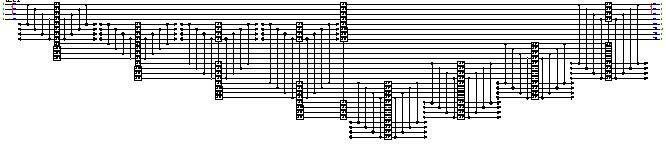
\includegraphics[width=0.5\textwidth]{img2.png}
\caption{The circuit for o4 POW17}
\end{figure}

\section{Scalability Test}
Seven non-trivial quantum algorithms were implemented in Quipper to demonstrate its scalability \cite{DBLP:journals/corr/abs-1304-3390}. This effort, involving 11 geographically dispersed programmers, resulted in functional representations suitable for realistic resource estimation.

\section{Architecture and Capabilities}
Quipper's architecture takes advantage of Haskell's type system to detect programming errors at compile time \cite{DBLP:journals/corr/abs-1304-3390}. Other important capabilities include the automatic creation of quantum oracles via 'circuit removal' and the manipulation of all sub-circuits, making them user-friendly.

\begin{figure}[h]
\centering
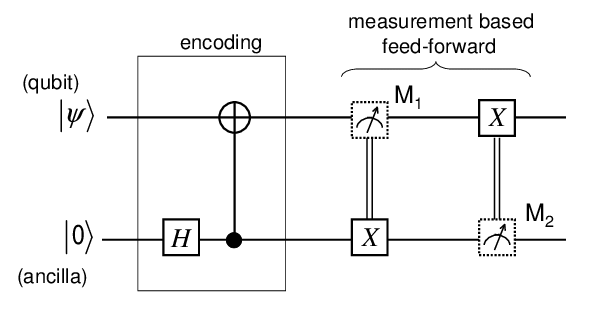
\includegraphics[width=0.5\textwidth]{img.png}
\caption{A visual representation of Quipper's architecture}
\end{figure}

\section{Optimization}
Quipper's optimisation capabilities are exemplified by the implementation of the Triangle Finding algorithm \cite{DBLP:journals/corr/abs-1304-3390}. The algorithm was optimised by reducing the number of gates and qubits, and a significant advance in quantum computing was achieved.

\section{Conclusion}
As a quantum programming language, Quipper achieves scalability suitable for expressing complex, large-scale quantum algorithms and enabling their optimisation \cite{DBLP:journals/corr/abs-1304-3390}. Future research aims to improve the functionality of Quipper, including further computational modelling, quantum error correction and integration with a quantum simulator.

\newpage

\bibliographystyle{plain}
\bibliography{literature.bib}

\end{document}
